\documentclass[10pt, titlepage]{report}

\usepackage[utf8]{inputenc}
\usepackage[T1]{fontenc}
\usepackage[francais]{babel}

%Caractères spéciaux

\usepackage{lmodern}
\usepackage{amsmath}
\usepackage{amssymb}
\usepackage{mathrsfs}

\usepackage{eurosym} %insertion signe euro
\usepackage{graphicx} %insertion d'images
\usepackage{fancyhdr} %en-tete et pied de page

\title{\bsc{Rapport de la deuxième soutenance}\\Projet flight arena}
\author{mr cube :\\
Vincent \bsc{Rospini-Clerici},\\
Guillaume \bsc{Rebut}\\
%Nikolas \bsc{Miletic}\\
chef de projet : Arthur \bsc{Remaud}}
\date{7 mai 2015}

\pagestyle{fancy}
\fancyhead{}
\fancyfoot{}
\lhead{Rapport de la deuxième soutenance}
\rhead{Projet flight arena}
\lfoot{mr cube}

\begin{document}

\maketitle
\renewcommand{\contentsname}{Sommaire}
\renewcommand{\chaptername}{Partie}

\tableofcontents

\chapter{Retard/Avance par rapport au cahier des charges}

\section{Prévisions}

\section{Retard}

\section{Avance}

\chapter{Travail par membre}
Nous allons vous décrire ce que chaque membre de l'équipe mr cube a fait pendant cette deuxième période, avec leurs difficultés rencontrées et les techniques utilisées.

\section{Guillaume Rebut}

\subsection{Ce que Guillaume doit faire pour la seconde soutenance}

\section{Vincent Rospini-Clerici}

\subsection{Différents problèmes rencontrés}

\subsection{Ce que Vincent doit faire pour la seconde soutenance}

\section{Arthur Remaud}

\subsection{Multijoueur en réseau}
Pendant cette période, Arthur a surtout travaillé sur le multijoueur. Il a d'abord essayé de faire un protocole UDP pour relier en LAN (Local Area Network) en s'inspirant du TP que nous avions fait lorsque nous avions travaillé sur le protocole TCP, avant de se rendre compte qu'il existait la classe Network sur Unity. Plusieurs tutoriels existent à ce sujet sur internet, Arthur s'en est donc inspiré pour faire un réseau où le joueur peut choisir d'héberger une partie ou d'en rejoindre une à partir de son adresse IP locale.\\

Le principal problème fut qu'au départ, les joueurs contrôlaient le vaisseau de l'autre joueur et donc devait regarder sur l'autre écran pour jouer. De plus, à trois joueurs, les deux premiers connectés voyaient un seul et même vaisseau qu'il contrôlaient tous les deux pendant que le troisième joueur en pilotait un autre. Le dernier vaisseau quant à lui n'était contrôlé par personne et restait immobile. Au final, ce problème venait de l'assignation des caméras et des scripts aux joueurs lorsqu'ils instanciaient un nouveau vaisseau en arrivant.

\subsection{Quaternions}
Il nous avait été demandé à la dernière soutenance de modifier les déplacements des vaisseaux en rajoutant des quaternions. Comme c'était Arthur qui s'était chargé des mouvements à la base, c'est lui qui a modifié le code pour mettre à la place des quaternions. Maintenant, les mouvements sont plus réalistes grâce à l'inertie mais cela rend le jeu un peu plus difficile.\\

Parfois, lorsque le vaisseau tournaient longtemps sur lui-même, il se mettait soudainement à partie dans l'autre sens avant de repartir de la rotation voulue. En effet le quaternion dépassait les 180\textdegree  et donc la rotation s'inversait. En ajoutant un maximum à l'accélération, on a pu régler facilement ce petit imprévu.

\subsection{Intelligence artificielle}

Arthur a commencé à faire une intelligence artificielle pour pouvoir jouer contre des vaisseaux contrôlés par l'ordinateur. Pour le début nous voulions faire un algorithme de pathfiding. Cependant la 3D nous posait problème, car on ne peut représenter facilement le terrain sous forme de tableau. Il faudrait utiliser un graphe, mais non seulement nous ne savons pas comment le faire, mais en plus il faudrait en faire un différent pour chaque carte.\\

Nous avons donc opté pour une autre technique : devant le vaisseau, nous avons rajouté des cylindres invisibles qui détectent des collisions avec les murs. Lorsque cela se produit, le vaisseau tourne alors en conséquence pour ne pas rentré dans l'obstacle.

\subsection{Menus}

Le menu a été complété par Arthur. Il a rajouté la sélection de la qualité d'image dans le menu option pour pouvoir choisir en fonction de la performance de son ordinateur les meilleurs graphismes possibles.\\

Il a aussi fait en sorte que le joueur puisse choisir le vaisseau qu'il veut piloter parmi les différents proposés avant de commencer la partie.\\

Au départ, nous voulions faire en sorte que le joueur puisse choisir la répartition des touches de son clavier s'il voulait changer ses commandes. Cependant, nous ignorons totalement comment le faire et nous ne trouvons rien sur internet pour le faire, même dans la documentation de Unity. Nous avons donc abandonné cette idée.

\subsection{Ce qu'Arthur doit faire pour la prochaine soutenance}

\chapter{Pour la prochaine soutenance}


bla\\ \\ \\ \\ \\ \\ \\

\begin{center}
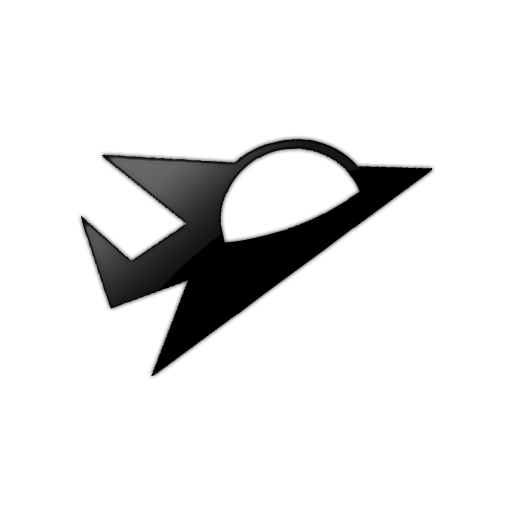
\includegraphics[height=4cm, width=4cm]{vaisseux_petit.png}
\end{center}

\end{document}